% Hình hợp đồng thời gian; nguồn và binding nằm tại thesis/evidence.md mục 8.4.
% Biên dịch riêng bằng pdfLaTeX; PDF vector có thể chèn vào nguồn toàn văn sau.
\documentclass[10pt]{article}
\usepackage[T1]{fontenc}
\usepackage{lmodern}
\usepackage[paperwidth=170mm,paperheight=112mm,margin=4mm]{geometry}
\usepackage{tikz}
\usetikzlibrary{arrows.meta,calc}
\pagestyle{empty}
\setlength{\parindent}{0pt}
\definecolor{history}{HTML}{EAF2F8}
\definecolor{future}{HTML}{FFF1E7}
\definecolor{ink}{HTML}{1F3445}
\definecolor{accent}{HTML}{126B80}
\definecolor{warm}{HTML}{9A4D16}
\begin{document}
\centering
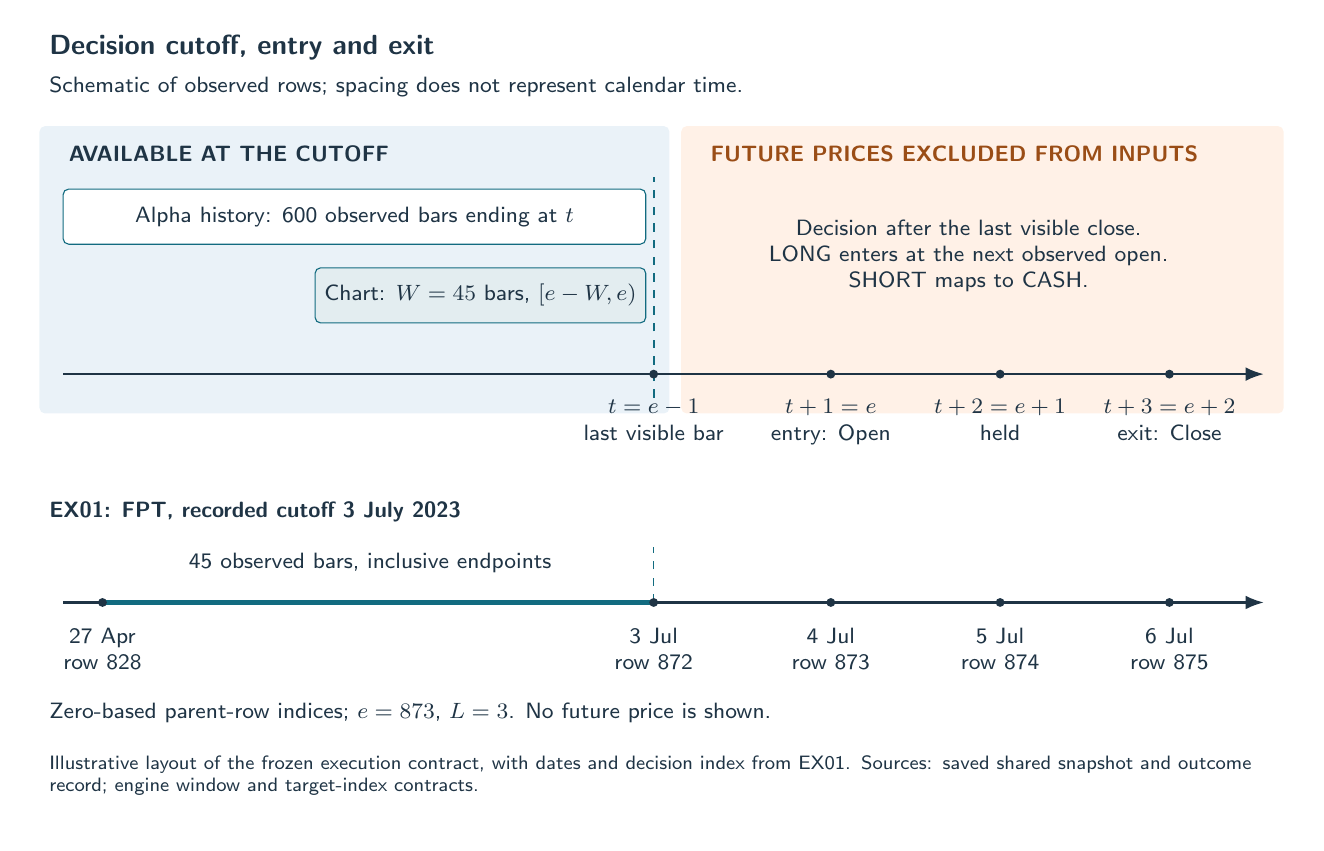
\begin{tikzpicture}[x=1cm,y=1cm,>=Latex,font=\sffamily\small,text=ink]
  \path[use as bounding box] (0,0) rectangle (16.1,10.1);
  \node[anchor=west,font=\sffamily\bfseries] at (.15,9.85)
    {Decision cutoff, entry and exit};
  \node[anchor=west,font=\sffamily\footnotesize] at (.15,9.35)
    {Schematic of observed rows; spacing does not represent calendar time.};

  \fill[history,rounded corners=2pt] (.15,5.2) rectangle (8.15,8.85);
  \fill[future,rounded corners=2pt] (8.3,5.2) rectangle (15.95,8.85);
  \node[anchor=west,font=\sffamily\bfseries\footnotesize] at (.4,8.5)
    {AVAILABLE AT THE CUTOFF};
  \node[anchor=west,font=\sffamily\bfseries\footnotesize,text=warm] at (8.55,8.5)
    {FUTURE PRICES EXCLUDED FROM INPUTS};
  \draw[accent,fill=white,rounded corners=2pt] (.45,7.35) rectangle (7.85,8.05);
  \node[font=\sffamily\footnotesize] at (4.15,7.7)
    {Alpha history: 600 observed bars ending at $t$};
  \draw[accent,fill=accent!12,rounded corners=2pt] (3.65,6.35) rectangle (7.85,7.05);
  \node[font=\sffamily\footnotesize] at (5.75,6.7)
    {Chart: $W=45$ bars, $[e-W,e)$};
  \node[align=center,font=\sffamily\footnotesize] at (11.95,7.2)
    {Decision after the last visible close.\\
     LONG enters at the next observed open.\\
     SHORT maps to CASH.};
  \draw[ink,->,thick] (.45,5.7) -- (15.7,5.7);
  \draw[accent,dashed,thick] (7.95,5.4) -- (7.95,8.2);
  \foreach \x in {7.95,10.2,12.35,14.5}
    \fill[ink] (\x,5.7) circle (1.6pt);
  \node[align=center,anchor=north,font=\sffamily\footnotesize] at (7.95,5.5)
    {$t=e-1$\\last visible bar};
  \node[align=center,anchor=north,font=\sffamily\footnotesize] at (10.2,5.5)
    {$t+1=e$\\entry: Open};
  \node[align=center,anchor=north,font=\sffamily\footnotesize] at (12.35,5.5)
    {$t+2=e+1$\\held};
  \node[align=center,anchor=north,font=\sffamily\footnotesize] at (14.5,5.5)
    {$t+3=e+2$\\exit: Close};

  \node[anchor=west,font=\sffamily\bfseries\footnotesize] at (.15,3.95)
    {EX01: FPT, recorded cutoff 3 July 2023};
  \draw[ink,->,thick] (.45,2.8) -- (15.7,2.8);
  \draw[accent,line width=2pt] (.95,2.8) -- (7.95,2.8);
  \draw[accent,dashed] (7.95,2.8) -- (7.95,3.5);
  \foreach \x in {.95,7.95,10.2,12.35,14.5}
    \fill[ink] (\x,2.8) circle (1.6pt);
  \node[anchor=south,font=\sffamily\footnotesize] at (4.35,3.05)
    {45 observed bars, inclusive endpoints};
  \node[align=center,anchor=north,font=\sffamily\footnotesize] at (.95,2.6)
    {27 Apr\\row 828};
  \node[align=center,anchor=north,font=\sffamily\footnotesize] at (7.95,2.6)
    {3 Jul\\row 872};
  \node[align=center,anchor=north,font=\sffamily\footnotesize] at (10.2,2.6)
    {4 Jul\\row 873};
  \node[align=center,anchor=north,font=\sffamily\footnotesize] at (12.35,2.6)
    {5 Jul\\row 874};
  \node[align=center,anchor=north,font=\sffamily\footnotesize] at (14.5,2.6)
    {6 Jul\\row 875};
  \node[anchor=west,font=\sffamily\footnotesize] at (.15,1.4)
    {Zero-based parent-row indices; $e=873$, $L=3$. No future price is shown.};
  \node[anchor=west,align=left,text width=15.6cm,font=\sffamily\scriptsize] at (.15,.6)
    {Illustrative layout of the frozen execution contract, with dates and decision index from EX01.
     Sources: saved shared snapshot and outcome record; engine window and target-index contracts.};
\end{tikzpicture}
\end{document}
